% proj5.tex
% ITY 2017/2018
% Filip Kocica xkocic01@fit.vutbr.cz
% 15/4/2017

\documentclass[fyma2,pdf,final]{prosper}

\usepackage[czech]{babel}
\usepackage[utf8]{inputenc}
\usepackage[T1]{fontenc}
\usepackage{picture}
\usepackage{graphics}

\slideCaption{\textit{\textbf{proj5.tex} -- Typografie a publikování 2017/2018 -- Filip Kočica -- 15.4.2017}}
\DefaultTransition{Wipe}

\begin{document}

%\slideCaption{ITY -- proj5}
\title{\TeX}
\subtitle{ITY -- Projekt č. 5}
\author{Filip Kočica}
\email{xkocic01@fit.vutbr.cz}
\institution{Vysoké učení technické v~Brně\\Fakulta informačních technologií}
\maketitle

\begin{slide}{Autor \TeX u}
\begin{itemize}
    \item Donald Ervin Knuth (* 10.1.1938 USA). \bigskip
    \item Informatik a emeritní profesor na Stanfordově univerzitě. \bigskip
    \item Je autor díla \emph{Umění programování}, při kterém vytvořil \TeX. \bigskip
    \item Průkopník oboru matematické analýzy algoritmů, ale významně ovlivnil
          i~další informatické obory, například tvorbu překladačů nebo zpracování textu.
    \begin{center}
      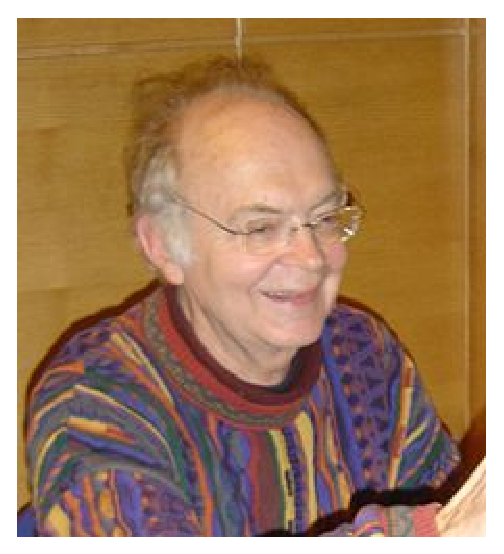
\includegraphics[width=0.3\textwidth]{donald_e_knuth.eps}
    \end{center} \bigskip
\end{itemize}
\end{slide}

\begin{slide}{Vznik a vývoj \TeX u}
\begin{itemize}
    \item Knuth nebyl spokojen s kvalitou vysázení skript pro studenty. \bigskip
    \item V té době nízká kvalita typografických prostředků. \bigskip
    \item Odhad doby vývoje \TeX u byl 6 měsíců, ovšem nakonec trval 10 let. \bigskip
    \item Způsob označování verzí programu není tradiční zvyšování čísla verze,ale verze
          TeXu se prodlužuje o další číslici desetinného rozvoje Ludolfova čísla. \bigskip
    \item Důraz kladen na korektní typografická pravidla a sazbu matematiky.
\end{itemize}
\end{slide}

\begin{slide}{Soubory maker pro \TeX}
\begin{table}[h!]
\begin{center}\catcode`\-=12
\begin{tabular}{|c|c|c|}\hline
\textbf{Balík maker} & \textbf{Vznik} & \textbf{Autor/Autoři}\\ \hline
   LaTeX & 1985 & Leslie Lamport\\ \hline
   BiBTeX & 1985 & Oren Patashnik a Leslie Lamport\\ \hline
   AmSTeX & 1983 & Michael Spivak\\ \hline
   PlainTeX & 1983 & Donald E. Knuth\\ \hline
\end{tabular}
\end{center}
\end{table}
\end{slide}

\overlays{5}{
\begin{slide}{Popis procesu kompilace}

\begin{itemstep}
    \item Načtě se .tex soubor a vytvoří se .dvi
	  \item \textbf{dvi2ps} převede .dvi na .ps
    \item \textbf{ps2pdf} převede .ps na .pdf
    \item \textbf{pdflatex} převede přímo .tex na .pdf
    \item
\begin{itemize}
    \item PS -- Post Script (Interpretovaný jazyk pro grafický popis dokumentů pro tisk.) \bigskip
    \item DVI -- Device Independent (Obsahuje binární data popisující vzhled dokumentu.) \bigskip
\end{itemize}
\end{itemstep}
\end{slide}
}

\begin{slide}{Proces kompilace graficky}
\begin{figure}[ht]
\begin{picture}(320,200)
\linethickness{1pt}

    \put(20,140){\framebox(60,20){\shortstack{\LaTeX}}}

   \put(130,140){\framebox(60,20){\shortstack{DVI}}}
   \put(80,150){\vector(2,0){50}}
   \put(95,160){{\shortstack{\LaTeX}}}

   \put(240,140){\framebox(60,20){\shortstack{PostScript}}}
   \put(190,150){\vector(2,0){50}}
   \put(205,160){{\shortstack{dvips}}}

   \put(240,70){\framebox(60,20){\shortstack{PDF}}}
   \put(270,140){\vector(0,-2){50}}
   \put(238,113){{\shortstack{ps2pdf}}}

\end{picture}
\end{figure}
\end{slide}

\begin{slide}[Split]{Použité zdroje}
\begin{itemize}
    \item https://en.wikipedia.org/wiki/LaTeX
    \item https://en.wikipedia.org/wiki/TeX
    \item http://wiki.vavricek.cz/images/2/25/ELP-prez-ste446-historie.pdf
    \item https://en.wikibooks.org/wiki/LaTeX/Basics\#Compilation\_process
\end{itemize}
\end{slide}

\begin{slide}{}
\vspace{42pt}
\begin{center}
  {\large Děkuji za pozornost}
\end{center}
\end{slide}

\end{document}
